\chapter{Appendix}
\section{Symbols}
\label{sec:symbols}
\begin{tabular}{p{2cm} l}
$I_{x}$ & Identity matrix of dimension \emph{x} \\
$\textbf{0}_{r \times c}$ & Zero matrix of dimensions given by \emph{r,c}. \\
						  & \emph{r} - row dimension , \emph{c} - colomn dimension \\
$e_i$ 			& Unit vectors pointing in direction of the coordinate axis  \\
				& $e_1 = \begin{bmatrix} 1 \\ 0 \\ 0 \end{bmatrix} $ - unit vector along x axis \\						& $e_2 = \begin{bmatrix} 0 \\ 1 \\ 0 \end{bmatrix} $ - unit vector along y axis \\						& $e_3 = \begin{bmatrix} 0 \\ 0 \\ 1 \end{bmatrix} $ - unit vector along z axis \\	
$l_{m,n}$    	& Zero vector of length \emph{m}, with 1 in \emph{nth} position of the vector \\
			    & For Example, $l_{4,2} = \begin{bmatrix} 0 \\ 1 \\ 0 \\ 0 \end{bmatrix}, l_{2,1} = 						\begin{bmatrix} 1 \\ 0 \end{bmatrix} $ \\		
\end{tabular}

\section{Abbreviation}
\begin{tabular}{c l}
EKF & Extended Kalman filter \\
IMU & Inertial measurement Unit \\
FTS & Force torque sensor \\
ODE & Ordinary differential equation\\
ZMP & Zero moment point\\
RPY & Roll-Pitch-Yaw
\end{tabular}

\section{Rotation matrix}
\label{sec:rot_mat}
The orientation of a rigid body in space can be represented in form of rotational matrix $R \in SO(3)$. 
\begin{figure}
    \centering
    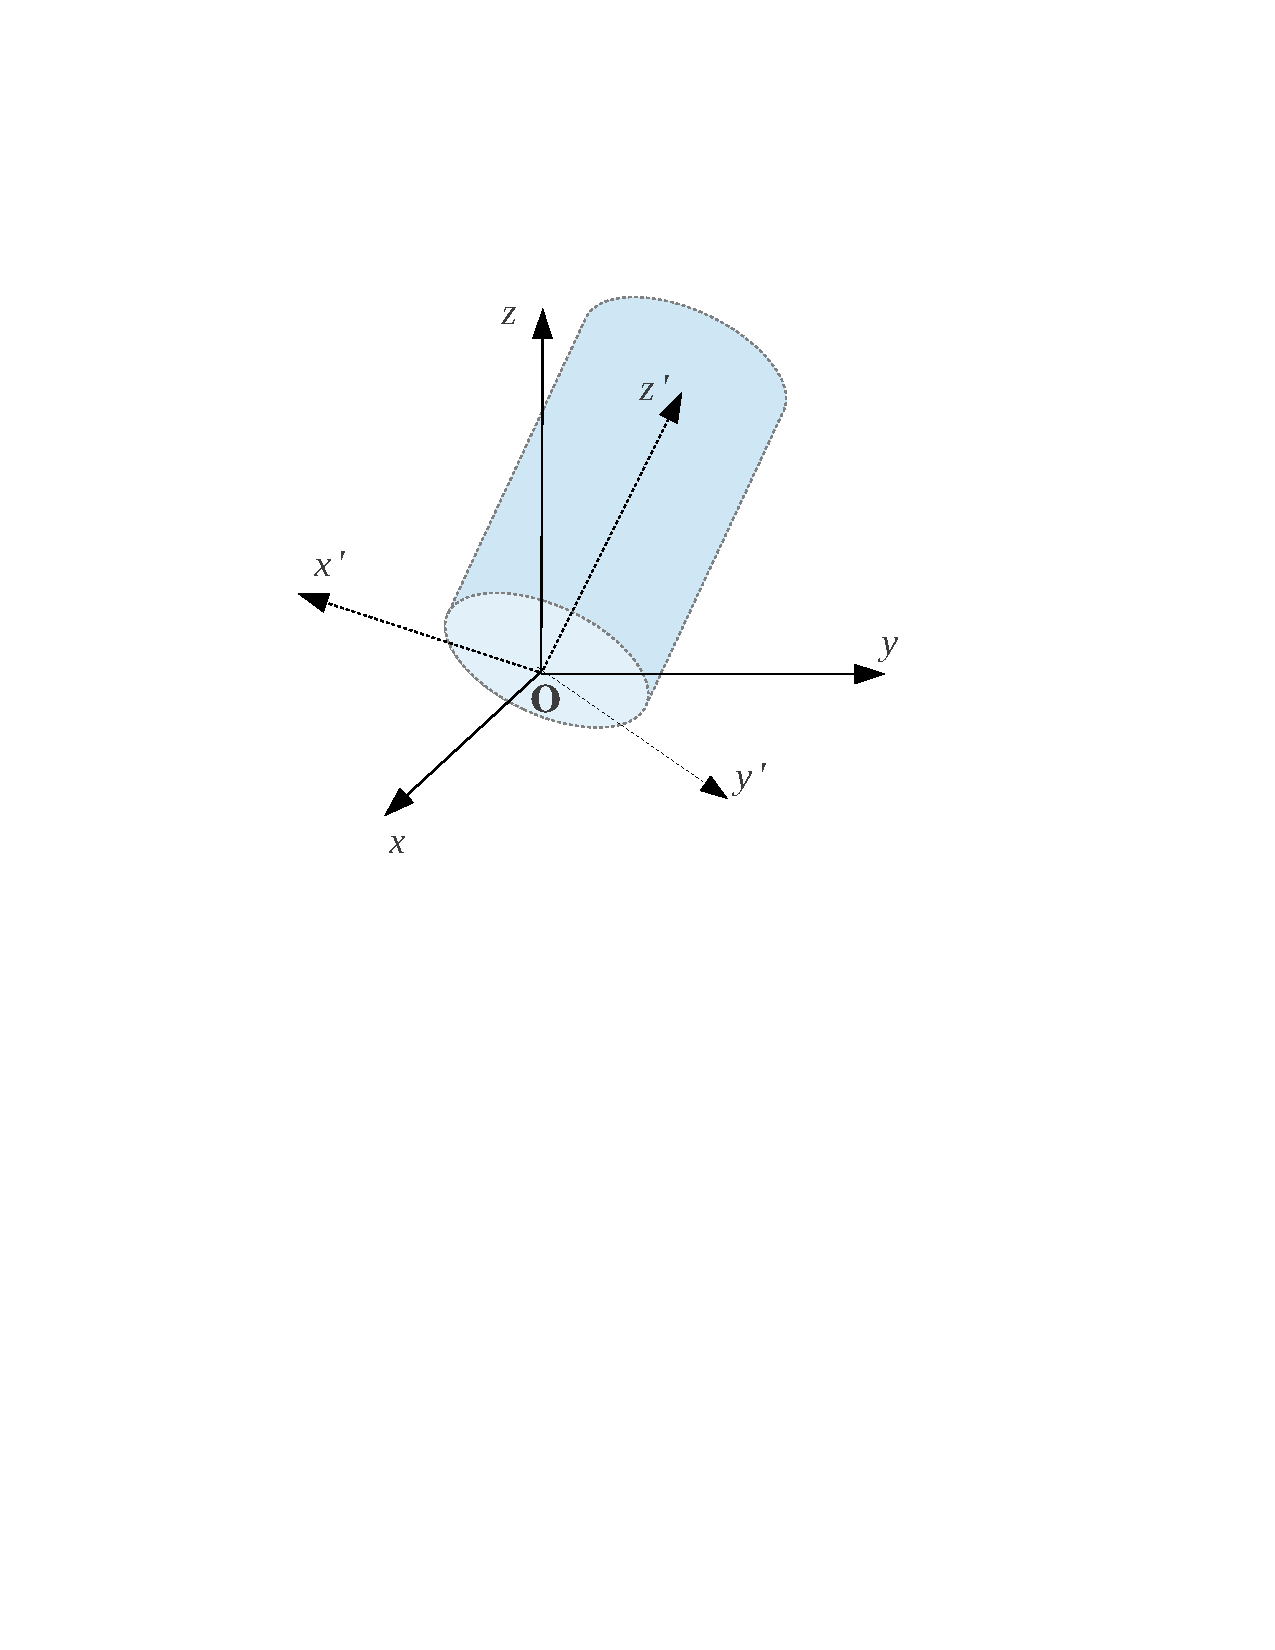
\includegraphics[trim = 5cm 13cm 5cm 5cm, scale = 0.65]{Bilder/rot_ab.pdf}
    \caption{Rotation of a rigid body about a point}
    \label{fig:rot_ab}
\end{figure}
Figure \ref{fig:rot_ab} shows the cylindrical object rotated about point \textbf{O}. \emph{x',y',z'} are the frames attached to the cylindrical object. The frame attached to the body of the object is denoted as frame \emph{B} \emph{x,y,z} represents the inertial frame or spatial frame and it is denoted as frame \emph{A}. The rotation of frame \emph{B} with respect to frame \emph{A} is given as $$ R_b^a.$$. In this thesis unless explicitly mentioned the rotation matrix represents the rotation of a body with respect to inertial frame or spatial frame. For the sake of simplicity in symbols the rotation of the body with respect to spatial frame is represented as $R$ instead of $R_b^a$.
A 3 dimensional rotation matrix defines the rotation along \emph{X,Y,Z} directions. The rotation matrix is composition of these individual rotations. The matrix representing the rotation around each coordinate axis is,
\begin{equation}
	\begin{split}
	R_x(\theta_x) = 
	\begin{bmatrix}
	1 &0 &0 \\ 0 &cos(\theta_x) &-sin(\theta_x)\\ 0 &sin(\theta_x) &cos(\theta_x)
	\end{bmatrix}\\
	R_y(\theta_y) = 
	\begin{bmatrix}
	cos(\theta_y) &0 &sin(\theta_y) \\ 0 &1 &0\\ -sin(\theta_y) &0 &cos(\theta_y)
	\end{bmatrix}\\
	R_z(\theta_z) = 
	\begin{bmatrix}
	cos(\theta_z) &-sin(\theta_z) &0 \\ sin(\theta_z) &cos(\theta_z) &0)\\ 0 &0 &1
	\end{bmatrix}
	\end{split}
\end{equation}
\begin{enumerate}
\item Rotation matrix for the whole body model in Chapter \ref{chap:multi_mdl} is 
\begin{equation}
	\label{eq:rot_full}
	\begin{split}
	R &= R_x(\theta_x) R_y(\theta_y) R_z(\theta_z) \\
	&= 
	\begin{bmatrix}
		c_yc_z &-c_ys_z &s_y \\
		c_xs_z+c_zs_xs_y &c_xc_z-s_xs_ys_z &-c_ys_x \\
  		s_xs_z-c_xc_zs_y &c_zs_x-c_xs_ys_z & c_xc_y \\
	\end{bmatrix}
	\end{split}
\end{equation}
The partial derivative of the above rotational matrix with respect to the angles is
\begin{equation}
	\begin{split}
	\dfdx{R}{\theta_x} &=
	\begin{bmatrix} 
		0 &0 &0 \\
        c_xs_yc_z-s_xs_z &-c_xs_ys_z-s_xc_z &c_xc_y]\\
        s_xs_yc_z+c_xs_z &-s_xs_ys_z+c_xc_z &-s_xc_y
	\end{bmatrix}\\
	\dfdx{R}{\theta_y}&=
	\begin{bmatrix}
    -s_yc_z &s_ys_z &c_y \\
     s_xc_yc_z &-s_xc_ys_z & s_xs_y \\
    -c_xc_yc_z & c_xc_ys_z &-c_xs_y
	\end{bmatrix}\\
	\dfdx{R}{\theta_z}&=
	\begin{bmatrix}
    -c_ys_z &-c_yc_z &0 \\
    -s_xs_ys_z+c_xc_z &-s_xs_yc_z-c_xs_z &0 \\
     c_xs_ys_z+s_xc_z &c_xs_yc_z-s_xs_z &0
	\end{bmatrix}
	\end{split}
\end{equation}
\item Rotation matrix for the simplified model in Chapter \ref{chap:simp_mdl} is parameterized as RPY angles
\begin{equation}
	\label{eq:rot_simp}
	\begin{split}
		R &= R_z(\theta_z) R_y(\theta_y) R_x(\theta_x)\\ &=
		\begin{bmatrix}
		c_zc_y &-s_zc_x+c_zs_ys_x &s_zs_x+c_zs_yc_x\\
		s_zc_y &c_zc_x+s_zs_ys_x &-c_zs_x+s_zs_yc_x\\
		-s_y &c_ys_x &c_yc_x
		\end{bmatrix}
	\end{split}
\end{equation}
The partial derivative of the above rotational matrix with respect to the angles is
\begin{equation}
	\begin{split}	
		\dfdx{R}{\theta_x} &=
		\begin{bmatrix}
		0 &s_zs_x+c_zs_yc_x &s_zc_x-c_zs_ys_x \\
		0 &-c_zs_x+s_zs_yc_x &-c_zc_x-s_zs_ys_x \\
		0 &c_yc_x &-c_ys_x
		\end{bmatrix}\\
		\dfdx{R}{\theta_y} &=
		\begin{bmatrix}
		-c_zs_y &c_zc_ys_x &c_zc_yc_x \\
		-s_zs_y &s_zc_ys_x &s_zc_yc_x \\
		-c_y &-s_ys_x &-s_yc_x
		\end{bmatrix}\\
		\dfdx{R}{\theta_z} &=
		\begin{bmatrix}
		-s_zc_y &-c_zc_x-s_zs_ys_x &c_zs_x-s_zs_yc_x \\
		c_zc_y &-s_zc_x+c_zs_ys_x &s_zs_x+c_zs_yc_x\\
		0 &0 &0
		\end{bmatrix}
	\end{split}
\end{equation}
\begin{itemize}
\item $ \theta_x, \theta_y, \theta_z $ represents the rotation of the body coordinate frame relative to spatial frame coordinate frame.
\item $ c_x,c_y,c_z $ are the short hand notations of $cos(\theta_x), cos(\theta_y), c_z$ respectively.
\item $ s_x,s_y,s_z $ are the short hand notations of $sin(\theta_x), sin(\theta_y), sin(\theta_z)$ respectively.
\end{itemize}
\end{enumerate}
\section{ Homogeneous transformation matrix}
\label{sec:htm}
Homogeneous transformation matrix is a one form of representation of rigid body transformation. It represents the transformation of a rigid body from the body coordinate frame to another cooridnate frame. 
\begin{figure}
    \centering
    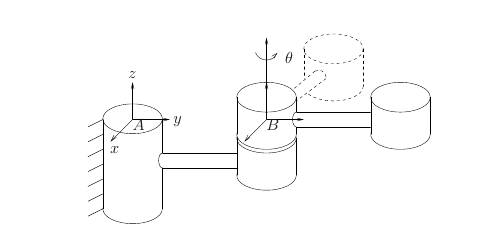
\includegraphics{Bilder/htm_example.png}
    \caption[Rigid body motion generated by rotation about a fixed axis]{Rigid body motion generated by rotation about a fixed axis \footnotemark[1]}
    \label{fig:htm}
\end{figure}
\footnotetext[1]{Source: A mathematical introduction to rigid body manipulation \citep[Chapter 2]{mur94}}
Homogeneous transformation matrix of body frame \emph{B} with respect to fixed frame \emph{A} is given as
\begin{equation}
    H_b^a = \begin{bmatrix} R_b^a(\theta) & p_{ab} \\ \textbf{0}_{3,1} &1 \end{bmatrix} \in SE(3),
\end{equation}
where $H_b^a$ represents the rigid body transfrormation of frame \emph{b} with respect to frame \emph{a}.
\begin{itemize}
    \item $R_b^a(\theta)$ is the rotation matrix representing rotation of body frame \emph{B} with respect to frame \emph{A}. 
    \item $p_{ab} = \begin{bmatrix} p_x \\ p_y \\ p_z \end{bmatrix} = \begin{bmatrix} p_1 \\ p_2 \\ p_3 \end{bmatrix} $ is the position of the body frame relative to spatial frame. 
\end{itemize}
For the sake of simplicity the homogeneous transofrmation matrix of a body with respect to spatial frame is represented by $H$ instead of $H_b^a$, the position as $p$ and rotation matrix as $R$.
The partial derivative of homogeneous transformation matrix with respect to poition and orientation.
\begin{equation}
    \begin{split}
    \dfdx{H}{p_i} &= \begin{bmatrix} \textbf{0}_{3,3} &e_i \\ \textbf{0}_{1,3} &1 \end{bmatrix} \hspace{2cm} i={1,2,3} \\
    \dfdx{H}{\theta_i} &= \begin{bmatrix} \dfdx{R}{\theta_i} &\textbf{0}_{3,1} \\ \textbf{0}_{1,3} &1 \end{bmatrix}
    \end{split}
\end{equation}

\section{Transformation of angular velocity to Euler rates}
\label{sec:avel_trfm}
The relation between the angular velocity and time derivative of rotational matrix is $$ \omega^b = (R^T \dot{R}) ^ \vee $$
\begin{itemize}
\item $\omega^b$ is the angular velocity of the body in represented in body coordinate frame. 
\item $R^T \dot{R}$ is a skew symmetric matrix \citep[Chapter 2]{mur94}.
$$ R^T \dot{R} = \begin{bmatrix}
0 &-\omega_z^b &\omega_y^b\\ \omega_z^b &0 &-\omega_x^b \\ -\omega_y^b &\omega_x^b &0 \end{bmatrix}$$
\item $\vee$ operator extracts the 3 dimensional vector that forms the skew symmetric matrix
$$ (R^T \dot{R}) ^ \vee = \begin{bmatrix}\omega_x^b\\ \omega_y^b\\ \omega_z^b \end{bmatrix} = w^b$$
\end{itemize}
The rotation matrix R is parametrized by Euler angles. $w^b$ depends on the parametrization of the rotation matrix.
\begin{enumerate}
\item For the whole body model discussed in Chapter \ref{chap:multi_mdl} the rotation matrix is given in Equation \ref{eq:rot_full}. The angular velocity is
\begin{equation}
	\begin{split}
	\omega_x^b &= cos(\theta_z)cos(\theta_y)\dot{\theta}_x + sin(\theta_z)\dot{\theta}_y \\
	\omega_y^b &= - sin(\theta_z)cos(\theta_y)\dot{\theta}_x + cos(\theta_z)\dot{\theta}_y \\
	\omega_z^b &= sin(\theta_y)\dot{\theta}_x + \dot{\theta}_z \\
	\begin{bmatrix}
	\omega_x^b\\ \omega_y^b\\ \omega_z^b
	\end{bmatrix}
	 &= 
	\begin{bmatrix}
		cos(\theta_z)cos(\theta_y) &sin(\theta_z) &0 \\
	 	-sin(\theta_z)cos(\theta_y) &c_z&0 \\
		sin(\theta_y) &0 &1
	\end{bmatrix}
	\begin{bmatrix}
			\dot{\theta_x} \\ \dot{\theta_y}\\ \dot{\theta_z}
	\end{bmatrix}\\
	& \omega^b = T(\theta) \dot{\theta}
	\end{split}
\end{equation}
$T(\theta)$ is the transformation matrix, that transforms the time derivative of euler angles parametrized in Equation \ref{eq:rot_full}.

The partial derivatives of $\omega^b$ with respect to the states are
$$\dfdx{\omega_b}{\theta_x} = \textbf{0}_{3\times 3},\dfdx{\omega_b}{\theta_y} = \begin{bmatrix}	-c_zs_y &0 &0\\ s_zs_y &0 &0\\ c_y &0 &0 \end{bmatrix}, \dfdx{\omega_b}{\theta_z} = \begin{bmatrix}	-s_zc_y &c_z &0\\ -c_zc_y &-s_z &0\\ 0 &0 &0 \end{bmatrix} $$

\item For the simple model discussed in Chapter \ref{chap:simp_mdl} the rotation matirx is given in Equation \ref{eq:rot_simp}. The angular velocity is
\begin{equation}
	\begin{split}
	\omega_x^b &= \dot{\theta}_x - sin(\theta_y)\dot{\theta}_z \\
	\omega_y^b &= cos(\theta_x)\dot{\theta}_y + cos(\theta_y)sin(\theta_x)\dot{\theta}_z \\
	\omega_z^b &= -sin(\theta_x)\dot{\theta}_y + cos(\theta_y)cos(\theta_x)\dot{\theta}_z \\
	\begin{bmatrix}
	\omega_x^b\\ \omega_y^b\\ \omega_z^b
	\end{bmatrix}
	 &= 
	\begin{bmatrix}
	 &1 &0 &-s_y\\
	 &0  &c_x &c_ys_x\\
	 &0  &-s_x &c_yc_x
	\end{bmatrix} \\
	&\omega^b = T(\theta) \dot{\theta}
	\end{split}
\end{equation}
$T(\theta)$ is the transformation matrix, that transforms the time derivative of euler angles parametrized in Equation \ref{eq:rot_simp}.

The partial derivatives of $\omega^b$ with respect to the states are
$$\dfdx{\omega_b}{\theta_y} = \begin{bmatrix}0 &0 &0\\ 0 &-s_x &c_yc_x\\ 0 &-c_x &-c_ys_x \end{bmatrix}, \dfdx{\omega_b}{\theta_z} = \begin{bmatrix}0 &0 &-c_y\\ 0 &0 &-s_ys_x\\ 0 &0 &-s_yc_x \end{bmatrix},\dfdx{\omega_b}{\theta_z} = \textbf{0}_{3\times 3} $$
\end{enumerate}
